\chapter{Caso d'uso}\label{chp:05-usecase}
%Dato il database di moon cloud con questi controlli e queste 
%evaluation si crea la seguente tassonomia. Dato un utente fresh che ha registrato target di 
%questo tipo l'algoritmo ritorna... Dato un altro utente nel db "simile"... così mettiamo tutto insieme.
\begin{figure}[ht!]
    \centering
    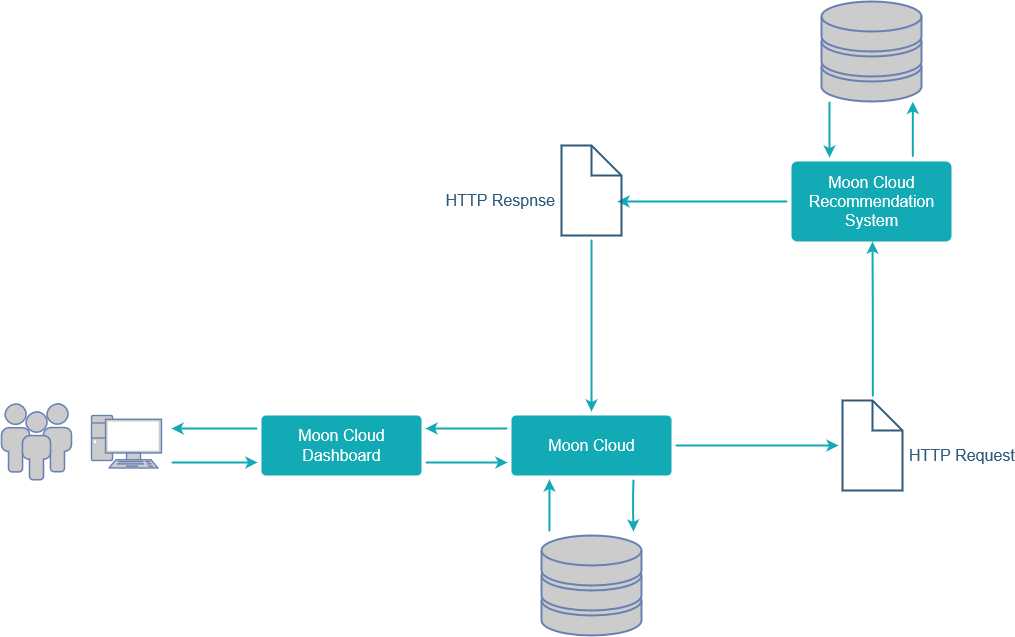
\includegraphics[scale=0.38]{images/UML_MoonCloud_HowToDo.png}
    \caption{.}
    \label{fig:UML_MoonCloud_HowToDo}
\end{figure}
%
Una volta implementato quanto proposto da questa tesi e integrato col sistema di Moon Cloud, nel momento in cui un utente 
accede ai servizi offerti da questo framework, completa la propria registrazione, uan copia dei suoi dati dal database di 
Moon Cloud verrà anche fatta nel database usato per poter effettuare il processo di recommendation; questa operazione di 
copia dei dati da una base di dati a un'altra viene fatta per poter avere i dati consistenti in entrambi i punti così da 
fornire al'utente delle raccomandazioni affidabili; ciò viene fatto non solo per i dati degli utenti ma anche per i Controlli 
e le Evaluation.\hfill\break
Inizialmente un nuovo utente, che ha appena effettuato la registrazione e avuto accesso alla propria dashboard, (l'interfaccia 
web) per poter schedulare e lanciare delle Evaluation, egli deve inserire uno o più Target (asset che l'utente possiede e su 
cui vuole essere certo che vengano rispette certe politiche di sicurezza o che vengano garantiti certi standard).\hfill\break
Nel momento in cui viene inserito il primo Target, del quale sarà specificato un Target Type (\textit{Url}, \textit{Host Windows}, 
\textit{Host Linux}, \textit{Azure} o \textit{Aws}), verra richiamato tramite l'apposita API REST (HTTP Request, method: GET, URL: 
\textit{recommendation/target/<str:target\_type\_id>/}) il \textit{Target Recommendation Algorithm}, il quale restituirà una 
risposta HTTP contenente, in formato JSON, una lista delle Evaluation ritenute più adatte per il Target specificato. Nel caso 
in cui l'utente ha inserito un Target di tipo \textit{Host Linux} nel Listing \ref{lst:rsp_Target_alg} è possibile trovare la risposta HTTP.
% ESEMPIO DI RICHIESTA E RISPOSTA - TARGET
\lstset{style=python_code_style}
\begin{lstlisting}[language=Python, label=lst:rsp_Target_alg, caption={URL: /recommendation/target/1/ }]
[
    {"other_id": 25},
    {"other_id": 29},
    {"other_id": 30},
    {"other_id": 24},
    {"other_id": 28},
    {"other_id": 31},
    {"other_id": 23},
    {"other_id": 26}
]
\end{lstlisting}